%!TeX program = xelatex
\documentclass[a4paper,UTF8,zihao=5]{ctexart}

\usepackage[left=2.45cm,right=2.45cm,top=2.45cm,bottom=2.45cm]{geometry}
\usepackage{amsmath,amssymb}
\usepackage{booktabs}
\usepackage{graphicx}
\usepackage{float}
\usepackage{tabularx}
\usepackage{array}
\usepackage{xcolor}
\usepackage{hyperref}
\usepackage{fancyhdr}
\usepackage{longtable}
\usepackage{caption}
\usepackage{subcaption}

\graphicspath{{figures/}}
\hypersetup{colorlinks=true,linkcolor=black,urlcolor=blue,citecolor=blue}
\urlstyle{tt}
\setlength{\headheight}{15pt}
\setlength{\emergencystretch}{3em}
\linespread{1.08}\selectfont
\setlength{\parindent}{2em}
\setlength{\parskip}{0.15em}
\setcounter{tocdepth}{2}
\pagestyle{fancy}
\fancyhead[L]{信息安全技术}
\fancyhead[C]{期末课程报告}
\fancyhead[R]{大语言模型文本水印}
\fancyfoot[C]{\thepage}
\captionsetup{font=small,labelfont=bf}
\renewcommand{\arraystretch}{1.14}

\newcommand{\cakl}{CA-KL}
\newcommand{\caklcg}{CA-KL-CG}
\newcommand{\kgw}{KGW}
\newcommand{\tpr}{TPR@1\%FPR}

\begin{document}

\begin{titlepage}
    \centering
    \vspace*{1.2cm}
    
\includegraphics[width=0.48\textwidth]{sysu.jpg}
    \vspace{1.8cm}

    {\zihao{2}\heiti 信息安全技术课程期末报告\par}
    \vspace{1.1cm}
    {\zihao{3}\heiti 基于逐 Token KL 约束与匹配检测的\par}
    \vspace{0.25cm}
    {\zihao{3}\heiti 大语言模型文本水印实验研究\par}
    \vspace{0.55cm}
    {\zihao{4} 基于 KGW 的复现、改进与 clean test-500 验证\par}

    \vfill
    \begin{tabular}{rl}
        学生姓名： & 施煌，祖裕柏，黄镇邦                 \\
        学号：   & 23336204，23344188，23342035 \\
        院系：   & 计算机学院                      \\
    \end{tabular}
    \vfill
    {\large 2026 年 7 月}
\end{titlepage}

\begin{abstract}
    本文面向大语言模型生成文本的来源识别问题，复现 Kirchenbauer 等人提出的 KGW 统计水印，并在统一、可审计的实验协议下研究逐位置 KL 约束水印。KGW 以固定偏置 $\delta$ 提高 green token 的采样概率，检测简单但无法直接约束不同上下文位置的分布扰动。为此，本文采用 \cakl{}：对每个生成位置求解满足 $D_{\mathrm{KL}}(Q_t\Vert P_t)\leq\varepsilon$ 的最大偏置 $\delta_t$，使水印强度由可解释的逐 token KL 预算控制；在完整方法 \caklcg{} 中进一步加入 candidate-aware greenlist、confidence gate 与配置严格匹配的 weighted detector。

    实验从 C4/realnewslike 构造互不重叠的 validation/test 各 500 条记录，在 OPT-1.3B、200 个生成 token、$\gamma=0.25$、temperature 1.0、top-k 0、top-p 1.0 的统一配置下完成参数选择与 test-500 $\times$ 3 seeds 独立评测。检测阈值由 validation human completions 校准；test human completions 的实际 FPR 为 0.6\%。不确定性采用 2,000 次 prompt-cluster bootstrap 估计。

    最终结果显示，\cakl{} 的 $\varepsilon$ 从 0.02 增至 0.50 时，\tpr{} 从 29.67\% 增至 99.53\%，同时 SimCSE 从 0.7218 降至 0.6566、corpus PPL 从 22.97 增至 34.14，呈现清晰的检测--质量折中。在预注册的 $\varepsilon=0.10$ 工作点上，\cakl{} 达到 94.80\% \tpr{}、0.6875 SimCSE 和 25.25 corpus PPL；KGW $\delta=1.0$ 为 92.27\%、0.6901 和 23.97。两条曲线在局部接近，但现有区间不足以支持“\cakl{} 严格改善 KGW Pareto 前沿”的强结论。对于 validation 选定的 \caklcg{}，standard KGW detector 的 TPR 为 86.40\%，matched weighted-global detector 则达到 97.80\%，表明检测配置与 candidate/gate 生成逻辑的一致性直接影响统计功效。总体而言，\cakl{} 提供了连续的检测--质量工作曲线，匹配检测显著恢复了完整方法的水印证据，但 clean 条件下尚不能宣称全面优于 KGW 固定偏置包络。

    \noindent\textbf{关键词：}大语言模型；文本水印；KGW；KL 散度；匹配检测；低误报率校准
\end{abstract}

\clearpage
\pagenumbering{Roman}
\tableofcontents
\clearpage
\pagenumbering{arabic}

\section{引言}

生成式大语言模型已经广泛进入写作、问答、教育和内容平台。模型文本与人工文本在表面形式上日益接近，使内容归属、批量生成识别和后续审计变得困难。文本水印的目标是在不增加可见标记的情况下，通过受密钥控制的生成概率偏置，在文本中留下可重复检验的统计证据。与训练一个通用 AI 文本分类器相比，生成式水印直接利用模型端密钥和生成过程，检测假设更明确，也更适合回答“该文本是否由某个受控模型生成”。

本文以 ICML 2023 的 KGW 水印为复现对象~\cite{kirchenbauer2023watermark}。原方法在每一步将词表按密钥划分为 greenlist 与 redlist，并给 greenlist logits 加固定偏置。固定偏置的优势是实现和统计量简单，但同一个 $\delta$ 在不同 next-token 分布上对应不同的真实扰动：模型非常确定时，推动其转向 green token 的代价可能很大；候选较多时，相同偏置又可能较温和。由此，本文研究逐位置 KL 预算能否比固定 $\delta$ 提供更可解释的检测--质量折中。

本文的主要工作如下：

\begin{enumerate}
    \item 完成 KGW 官方生成--检测链路复现，并保留其 seeded greenlist 与标准 z-score 作为共同基线；
    \item 建立结构化数据、全词表 greenlist、精确 PPL/SimCSE 计分、detector pairing 与 held-out calibration 组成的可复现实验流程；
    \item 在 test-500 $\times$ 3 seeds 上比较 7 个 KGW fixed-delta 点和 7 个 \cakl{} epsilon 点，并报告 held-out FPR、主质量指标和 prompt-cluster bootstrap 区间；
    \item 对 validation 选定的 \caklcg{} 与 matched KGW-CG 对照分别使用 standard、weighted-global 和 weighted-winmax 检测，分析生成逻辑与检测器匹配的作用。
\end{enumerate}

\section{KGW 方法与复现}

\subsection{Seeded greenlist 与固定偏置}

设基础语言模型在位置 $t$ 的条件分布为 $P_t(v)=P(v\mid x_{<t})$，词表为 $\mathcal V$。KGW 用密钥和前缀 $x_{<t}$ 产生伪随机种子，将 $\gamma|\mathcal V|$ 个 token 划入 greenlist $G_t$。若原 logits 为 $l_t(v)$，固定偏置生成分布使用
\[
    l'_t(v)=l_t(v)+\delta\,\mathbf 1[v\in G_t].
\]
检测端使用同一密钥逐位置重建 $G_t$。对长度为 $T$ 的待测文本，若观测到 $N_G$ 个 green token，则标准 KGW 统计量为
\[
    z=\frac{N_G-\gamma T}{\sqrt{T\gamma(1-\gamma)}}.
\]
无水印零假设下，green token 比例应接近 $\gamma$；显著偏高的 $z$ 支持水印假设。本文始终令 $\gamma=0.25$，并对 standard detector 的阈值在 validation human completions 上独立校准，而不是把固定的 $z>4$ 当作正式低 FPR 结论。可靠性研究同样强调阈值校准、误报率与文本长度的重要性~\cite{kirchenbauer2024reliability}。

\subsection{官方链路复现}

复现阶段按官方仓库完成最小模型和 OPT 模型的生成--检测链路验证，并处理新版 Gradio 的接口兼容问题。图~\ref{fig:official-demo} 展示了一次典型 Demo：无水印文本的 green fraction 为 22.2\%、$z=-0.638$；带水印文本的 green fraction 为 70.4\%、$z=10.4$。该结果确认密钥播种、greenlist 重建、logits 偏置与检测统计量能够端到端工作。

\begin{figure}[H]
    \centering
    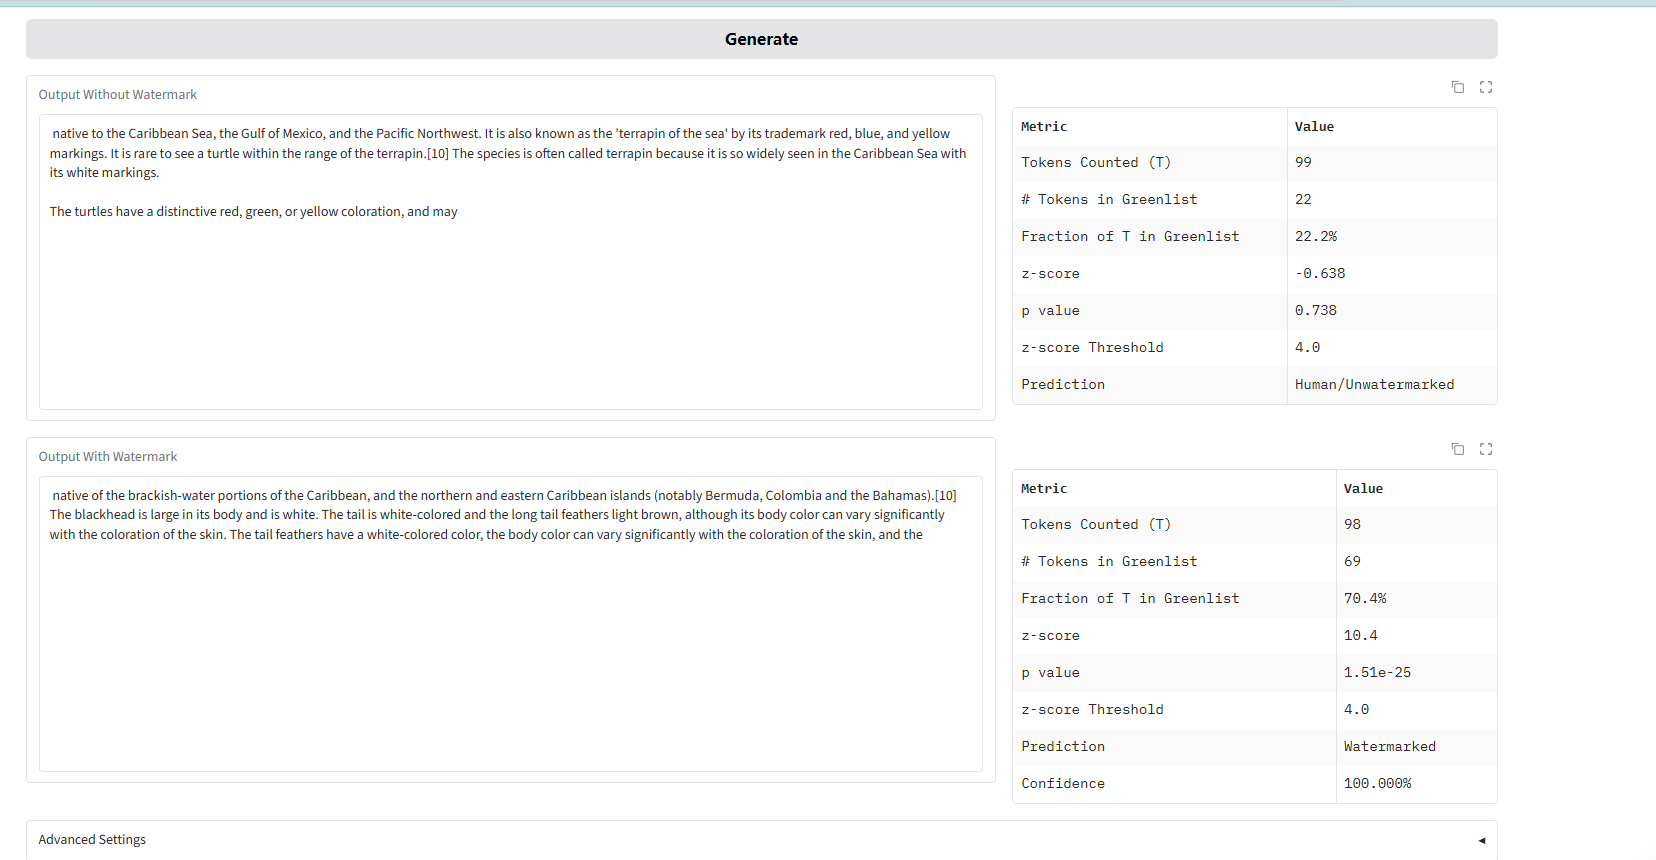
\includegraphics[width=0.88\textwidth]{official_demo_detection.png}
    \caption{KGW 官方 Demo 的生成与检测复现。}
    \label{fig:official-demo}
\end{figure}

\section{逐位置 KL 约束与匹配检测}

KGW 水印通过固定 logit 偏置提高 green token 的采样概率，其检测统计量简洁、可复现性强，但固定 $\delta$ 并不直接对应固定的分布扰动。对同一个 $\delta$，当基础模型在当前位置的分布更尖锐时，水印需要以更大的概率改变换取 green token 增益；当分布更平坦或候选 token 较多时，相同偏置造成的改变又相对温和。因此，本文将水印强度从固定偏置改写为逐位置 KL 预算，使每个生成位置的采样分布变化都由同一个可解释的上界控制，并进一步结合候选集合、置信门控和匹配检测器，使嵌入端与检测端围绕同一组条件分布完成统计判断。

在生成位置 $t$，基础语言模型首先给出条件分布 $P_t(v)=P(v\mid x_{<t})$；随后密钥和当前前缀共同确定可嵌入 token 的 greenlist，并由候选集合与置信门控决定当前位置是否施加水印。若该位置被选为可嵌入位置，算法求解满足逐 token KL 约束的最大偏置 $\delta_t$，据此得到水印采样分布 $Q_t$ 并生成下一个 token；若当前位置未通过门控，则保持原分布采样。检测时，检测器在相同密钥、相同基础模型和相同上下文下重建候选集合、greenlist、门控状态及其概率质量，并将每个位置的证据聚合为标准或加权统计量，最后用 validation human completions 校准的阈值判断文本是否含有水印。

\subsection{逐位置 KL 预算}

设原分布落在 greenlist 上的概率质量为
\[
    p_{G,t}=\sum_{v\in G_t}P_t(v).
\]
给 green token 加偏置 $\delta$ 后，归一化常数与新 green mass 分别为
\[
    Z_t(\delta)=1+p_{G,t}(e^{\delta}-1),\qquad
    q_{G,t}(\delta)=\frac{e^{\delta}p_{G,t}}{Z_t(\delta)}.
\]
加水印分布 $Q_{t,\delta}$ 相对原分布的正向 KL 为
\[
    D_{\mathrm{KL}}(Q_{t,\delta}\Vert P_t)
    =\delta q_{G,t}(\delta)-\log Z_t(\delta).
\]
\cakl{} 在每个位置通过二分搜索选择
\[
    \delta_t=\max\{\delta\in[0,\delta_{\max}]:
    D_{\mathrm{KL}}(Q_{t,\delta}\Vert P_t)\leq\varepsilon\},
\]
其中 $\delta_{\max}=3.0$，$\varepsilon$ 是逐 token 上限，而非整段文本的总预算。该约束直接限制当前采样分布相对基础分布的改变幅度，使水印强度具有明确的分布意义。

\cakl{} 的闭式 KL 定义在水印处理器接收的完整 softmax 分布上。实验采用 temperature 1.0、top-k 0 和 top-p 1.0，使处理器输出的 $Q_{t,\delta}$ 直接构成实际采样分布，避免后续温度缩放或候选截断改变概率支持集。在实现中，词表空间 $\mathcal V$ 以模型输出层定义，从而覆盖全部可采样 token；生成端与检测端在同一词表空间内执行密钥划分，保证 greenlist 重建的一致性。

\subsection{候选集合与置信门控}

仅在完整词表上划分 greenlist 会把一部分几乎不可能被采样的 token 纳入水印集合，导致有效证据与实际采样空间之间存在偏差。为此，本文引入 candidate-aware greenlist。令 $C_t$ 为按 $P_t(v)$ 降序排列后、累计概率首次达到 candidate top-p 的最小 token 集合，算法只在 $C_t$ 内依据密钥划分 green token，并在候选集合外保持原始采样概率。该设计使水印嵌入集中于模型当前真正可能选择的候选空间，减少低概率尾部 token 对统计证据的干扰。

置信门控用于进一步选择适合嵌入水印的位置。设 $g_t\in\{0,1\}$ 表示当前位置是否满足 entropy/top-1 条件：当基础分布过于确定或不满足预设置信条件时，算法令 $g_t=0$ 并取 $\delta_t=0$；当 $g_t=1$ 时，才在候选集合内求解逐位置 KL 约束下的偏置。候选集合决定水印划分的有效支持集，置信门控决定哪些位置参与嵌入，二者共同构成本文完整方法 \caklcg{}。

\subsection{匹配检测器}

当生成端使用候选集合或置信门控后，传统 KGW 检测器若仍按完整词表、全位置统计 green token，会与实际嵌入机制不完全一致。因此，本文使用 matched detector 作为完整方法的主要检测器：检测端逐位置重放基础模型分布，并在相同密钥下重建 $C_t$、$G_t$、$g_t$ 和 $p_{G,t}$。对于未通过门控的位置，检测器不将其作为有效水印证据；对于通过门控的位置，则按照重建后的候选空间计算 green token 偏离期望的程度。

一种一般化的 weighted z-score 可写为
\[
    z_w=\frac{\sum_t w_t(\mathbf 1[x_t\in G_t]-p_{G,t})}
    {\sqrt{\sum_t w_t^2p_{G,t}(1-p_{G,t})}},
\]
其中 $w_t$ 由模型分布和可嵌入性决定。Weighted-global 在全文范围内聚合证据；Weighted-WinMax 在多个滑动窗口上计算 $z_w$ 并取最大值。由于窗口搜索会引入多重比较效应，Weighted-WinMax 的阈值在 validation 集上独立校准，不与 standard 或 global 检测器共享阈值。本文的评测范围为 clean generation，WinMax 用于比较不同检测证据聚合方式的效果。

\section{实验设计}

\subsection{数据集与任务构造}

数据来自 C4/realnewslike~\cite{raffel2020exploring}。每条 source 经 OPT tokenizer 分词后保留 500--1000 token，末尾 200 token 作为 human completion，其前部保留 300--800 token 作为 prompt。数据以稳定 source ID 去重，并划分为互不重叠的 validation 与 test，各包含 500 条记录。validation 用于参数选择和检测阈值校准，test 用于最终性能评测。

\subsection{模型与参数设置}

生成模型为 \texttt{facebook/opt-1.3b}~\cite{zhang2022opt}，revision 为 \texttt{3f5c25d0bc631cb57ac65913f76e22c2dfb61d62}，FP16 推理。所有方法共享同一 prompt、生成长度、采样参数和 per-prompt 稳定 seed，配置见表~\ref{tab:config}。

\begin{table}[H]
    \centering
    \caption{实验模型、采样参数与工作点}
    \label{tab:config}
    \small
    \begin{tabular}{ll}
        \toprule
        项目                          & 冻结值                                                                      \\
        \midrule
        数据                          & C4/realnewslike；validation 500，test 500                                  \\
        Prompt / human / generation & 300--800 / 200 / 200 OPT tokens                                          \\
        Temperature / top-k / top-p & 1.0 / 0 / 1.0                                                            \\
        Greenlist 比例 / seeding      & $\gamma=0.25$ / \texttt{simple\_1}                                       \\
        KGW 网格                      & $\delta\in\{0.5,1.0,1.5,1.7,2.0,2.5,3.0\}$                               \\
        \cakl{} 网格                  & $\varepsilon\in\{0.02,0.05,0.10,0.20,0.30,0.40,0.50\}$，$\delta_{\max}=3$ \\
        完整方法                        & $\varepsilon=0.10$，candidate top-p=0.95，gate target=90\%                 \\
        Matched control             & KGW $\delta=1.5$，相同 candidate 与 gate                                     \\
        Test base seeds             & 1234，2345，3456                                                           \\
        \bottomrule
    \end{tabular}
\end{table}

\subsection{实验步骤}

实验按照以下四个步骤完成：

\begin{enumerate}
    \item 在小规模样本上验证 KGW、\cakl{} 与 matched detector 的实现一致性，包括固定生成长度、$\varepsilon=0$ 与 No-Watermark 等价、逐步 KL 约束、PPL continuation 边界以及 SimCSE 一一配对；
    \item 在 validation 集上扫描 KGW fixed-delta 与 \cakl{} epsilon 网格，并完成 candidate-only、gate-only 和 candidate+gate 消融，根据预设规则选择完整方法参数；
    \item 固定模型、采样参数、方法工作点、检测器配置和随机种子，在 500 条 test prompts 上以三个 base seeds 生成全部比较文本；
    \item 对冻结的 test 输出统一计算 standard/matched detector、corpus PPL 与 SimCSE，并使用 2,000 次 prompt-cluster bootstrap 估计 95\% 置信区间。
\end{enumerate}

\subsection{评价指标与统计方法}

主检测指标为 \tpr{}。每个 detector 均在 validation human completions 上以有限样本次序统计量确定阈值；test human completions 用于测量实际 FPR，test watermarked completions 用于测量 TPR。No-Watermark 模型文本的 model-null FPR 作为辅助统计量单独报告，human FPR 作为正式误报口径。standard KGW 的 1\% 目标阈值为 $z>2.4495$；test human FPR 为 0.6\%（95\% CI 0--1.4\%），No-Watermark model-null FPR 为 0.8\%（0.4--1.27\%）。

主语义指标为 continuation-only SimCSE cosine：对相同 prompt 和 seed，将水印 completion 与 No-Watermark completion 一一配对，使用 \texttt{princeton-nlp/sup-simcse-roberta-base} 自己的 tokenizer 和 pooler embedding。主分布质量指标为 continuation corpus PPL：
\[
    \operatorname{PPL}_{\mathrm{corpus}}=
    \exp\left(\frac{\sum_i \operatorname{NLL}_i}{\sum_i T_i}\right),
\]
只在生成 continuation 的精确 token IDs 上计分。图中的 mean row PPL 用于直观展示每条文本分布，主表使用 corpus PPL。

95\% CI 使用固定 calibration threshold 下的 2,000 次 prompt-cluster bootstrap。cluster 单位是 \texttt{prompt\_id}，同一 prompt 的三个 generation seeds 一起重采样，因而没有把 1,500 条重复测量误当成完全独立样本。区间反映 test prompt 抽样不确定性，不包含 validation threshold 的再次抽样不确定性。

\subsection{代码运行证明}

课程要求报告中包含代码运行效果截图。图~\ref{fig:code-run-proof} 展示批量实验脚本在服务器端完成多方法生成、结果文件保存、PPL 计算与校准指标输出的终端日志，其中包含最后一批 prompts 的处理进度以及结果 CSV、summary 与 calibrated metrics 的写入路径，可作为本文实验代码完整运行的证明。

\begin{figure}[H]
    \centering
    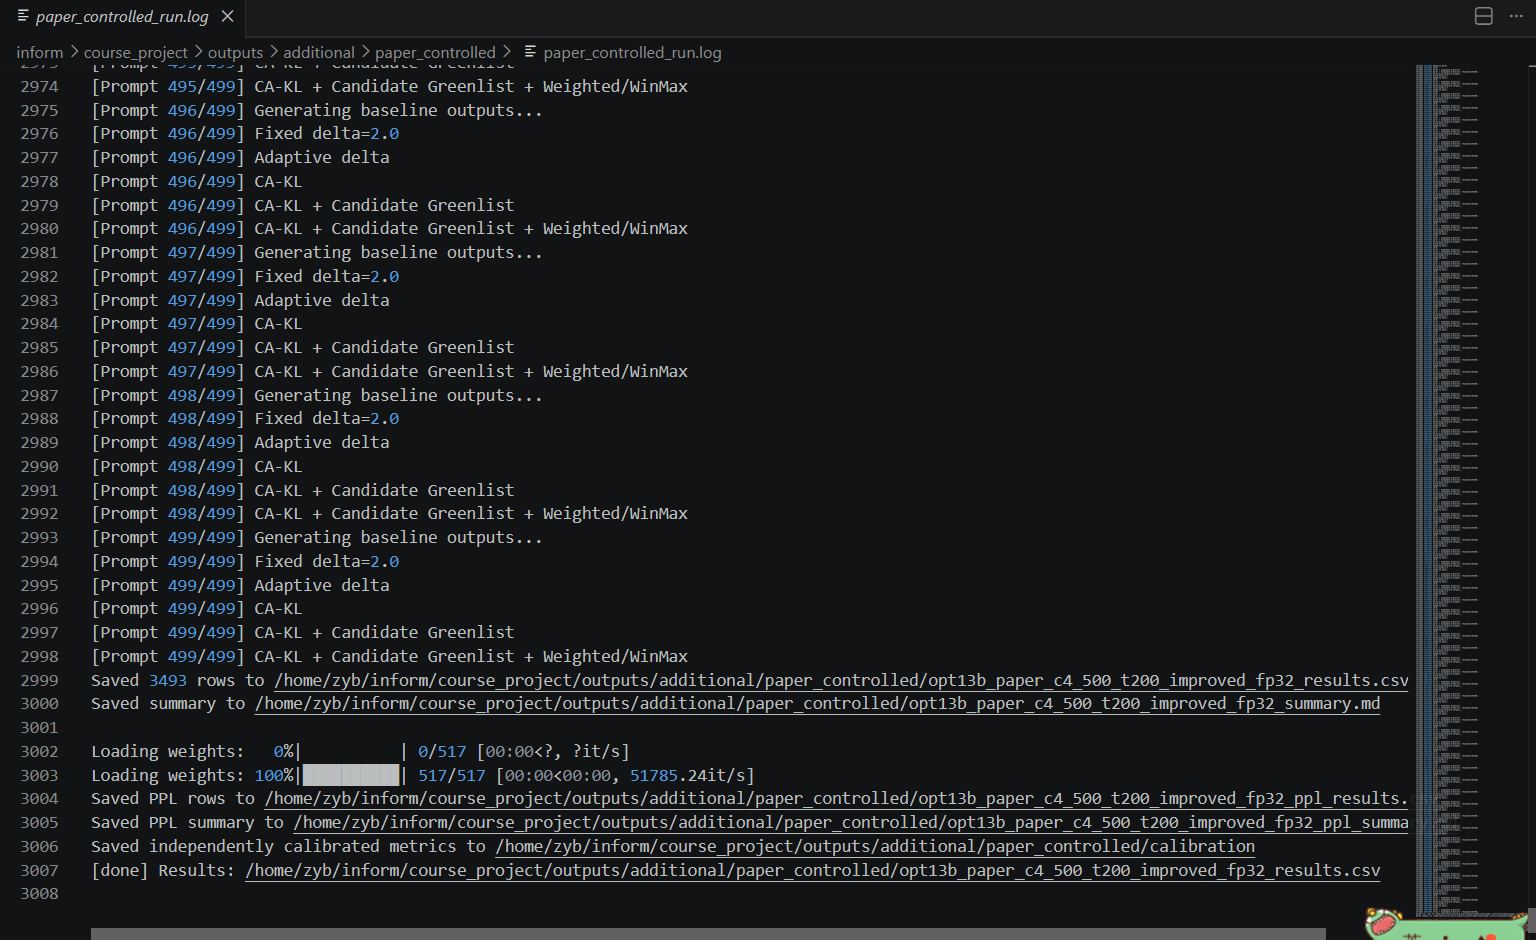
\includegraphics[width=\textwidth]{code_run_proof.png}
    \caption{代码运行效果截图：批量生成、PPL 计算与检测校准输出。}
    \label{fig:code-run-proof}
\end{figure}

\section{实验结果}

\subsection{Validation 集上的参数选择}

Validation 集上的完整网格表明，KGW 和 \cakl{} 均覆盖从约 30\% TPR 到接近饱和的弱、中、强水印区间。\cakl{} $\varepsilon=0.10$ 取得 97.6\% standard \tpr{}，SimCSE 为 0.6790，位于预注册的 95--98\% operating range，因而被选为 candidate/gate 消融的基础工作点；其余 epsilon 用于构建完整参数曲线。

Candidate-only 的 top-p=0.90、0.95、0.99 在 matched weighted-global detector 下的 validation TPR 分别为 99.0\%、99.2\%、98.8\%，对应 SimCSE 为 0.6842、0.6853、0.6781；因此选择 0.95。Gate-only 依据 No-Watermark validation 分布构造约 90\%、75\%、50\% 三种覆盖率。最终 candidate+gate 对比见表~\ref{tab:gate-selection}，按“先最大化 clean weighted-global \tpr{}，再比较 SimCSE”的规则选中 90\% gate。

\begin{table}[H]
    \centering
    \caption{Validation 集上 candidate top-p=0.95 的 gate 参数选择}
    \label{tab:gate-selection}
    \small
    \begin{tabular}{lrrrr}
        \toprule
        目标 gate pass & 实际含义   & Weighted-global TPR & SimCSE          & Mean row PPL    \\
        \midrule
        90\%         & 弱 gate & \textbf{99.0\%}     & 0.6852          & 26.086          \\
        75\%         & 中 gate & 98.8\%              & 0.6892          & 25.592          \\
        50\%         & 强 gate & 94.2\%              & \textbf{0.6956} & \textbf{25.230} \\
        \bottomrule
    \end{tabular}
\end{table}

90\% gate 的冻结阈值为 normalized entropy $H_{\min}=0.0067067$、top-1 probability $p_{\max}=0.9793311$。同时冻结 matched fixed-delta control：KGW $\delta=1.5$ 加相同 candidate top-p 与 gate。这样可区分动态 KL 与 candidate/gate、detector 本身的贡献。

\subsection{独立测试集上的 KGW 与 CA-KL}

Huo 等人的 token-specific watermarking 将 detectability 与 semantic coherence 作为联合优化目标，强调水印方法不能只用单一强度下的检测率判断，而应观察不同水印强度形成的检测--质量折中曲线~\cite{huo2024token}。受此评价方式启发，本文将 KGW fixed-delta 与 \cakl{} epsilon 扫描都视为一组 operating points：散点表示冻结 test 输出的实测结果，平滑曲线仅用于展示同一方法族内部随水印强度变化的趋势，不作为新的实验观测。

表~\ref{tab:main-test} 汇总 test-500 $\times$ 3 seeds 的 14 个主工作点。每个点的检测、SimCSE 和 PPL 样本均来自相同的 500 个 prompt；括号内为 95\% prompt-cluster bootstrap CI。

\begin{longtable}{p{0.12\textwidth}p{0.12\textwidth}p{0.225\textwidth}p{0.225\textwidth}p{0.225\textwidth}}
    \caption{独立测试集主工作点：standard KGW detector、SimCSE 与 corpus PPL}\label{tab:main-test}                  \\
    \toprule
    方法      & 参数                 & \tpr{}                & SimCSE                 & Corpus PPL          \\
    \midrule
    \endfirsthead
    \toprule
    方法      & 参数                 & \tpr{}                & SimCSE                 & Corpus PPL          \\
    \midrule
    \endhead
    \midrule
    \multicolumn{5}{r}{续下页}                                                                             \\
    \endfoot
    \bottomrule
    \endlastfoot
    KGW     & $\delta=0.5$       & 30.20\% [27.87,32.53] & 0.7248 [0.7173,0.7320] & 22.06 [21.17,23.00] \\
    KGW     & $\delta=1.0$       & 92.27\% [90.60,93.80] & 0.6901 [0.6820,0.6982] & 23.97 [22.99,24.97] \\
    KGW     & $\delta=1.5$       & 98.73\% [97.80,99.53] & 0.6761 [0.6679,0.6842] & 26.08 [25.06,27.11] \\
    KGW     & $\delta=1.7$       & 98.93\% [98.07,99.60] & 0.6729 [0.6647,0.6815] & 27.10 [26.01,28.29] \\
    KGW     & $\delta=2.0$       & 99.33\% [98.67,99.87] & 0.6636 [0.6556,0.6716] & 29.67 [28.52,30.86] \\
    KGW     & $\delta=2.5$       & 99.53\% [98.93,99.93] & 0.6610 [0.6533,0.6688] & 34.91 [33.58,36.37] \\
    KGW     & $\delta=3.0$       & 99.73\% [99.27,100]   & 0.6515 [0.6438,0.6592] & 41.37 [39.67,43.01] \\
    \midrule
    \cakl{} & $\varepsilon=0.02$ & 29.67\% [27.27,32.20] & 0.7218 [0.7143,0.7290] & 22.97 [22.03,23.94] \\
    \cakl{} & $\varepsilon=0.05$ & 70.47\% [68.00,73.07] & 0.7012 [0.6931,0.7088] & 24.22 [23.27,25.26] \\
    \cakl{} & $\varepsilon=0.10$ & 94.80\% [93.40,96.07] & 0.6875 [0.6791,0.6957] & 25.25 [24.27,26.29] \\
    \cakl{} & $\varepsilon=0.20$ & 98.80\% [98.07,99.40] & 0.6752 [0.6675,0.6830] & 28.25 [27.18,29.32] \\
    \cakl{} & $\varepsilon=0.30$ & 99.33\% [98.73,99.80] & 0.6692 [0.6611,0.6772] & 30.10 [29.00,31.28] \\
    \cakl{} & $\varepsilon=0.40$ & 99.60\% [99.07,100]   & 0.6678 [0.6603,0.6755] & 32.23 [31.04,33.45] \\
    \cakl{} & $\varepsilon=0.50$ & 99.53\% [98.93,99.93] & 0.6566 [0.6484,0.6645] & 34.14 [32.91,35.43] \\
\end{longtable}

在弱水印端，KGW $\delta=0.5$ 与 \cakl{} $\varepsilon=0.02$ 的 TPR 接近（30.20\% 对 29.67\%），前者同时具有略高 SimCSE 和略低 PPL。在中等工作点，\cakl{} $\varepsilon=0.10$ 相比 KGW $\delta=1.0$ 的 TPR 高 2.53 个百分点，但 SimCSE 低 0.0026、corpus PPL 高 1.28；相比 KGW $\delta=1.5$，其质量更好但 TPR 低 3.93 个百分点。这说明 \cakl{} 的改进不表现为单个点全面支配 KGW，而表现为用 $\varepsilon$ 给出更细粒度、可解释的 token-specific 强度调节，使检测率可以沿连续预算曲线逐步提高。

图~\ref{fig:sim-pareto} 聚焦 SimCSE $\leq0.69$、TPR 介于 0.94--1.00 的高检测区，以观察饱和区附近的 detectability--semantic coherence 前沿。高检测率附近，\cakl{} 的平滑趋势线与 KGW 曲线交错而非整体落后：例如 \cakl{} $\varepsilon=0.30$ 与 KGW $\delta=2.0$ 的 TPR 均为 99.33\%，但 SimCSE 分别为 0.6692 与 0.6636，前者高 0.0056；\cakl{} $\varepsilon=0.20$ 也在接近 98.8\% TPR 时保持 0.6752 的 SimCSE。该结果与 Huo 等人强调的 token-specific 折中视角一致，即改进重点在于按位置调节嵌入强度，而不是把所有位置推向同一个固定偏置。

\begin{figure}[H]
    \centering
    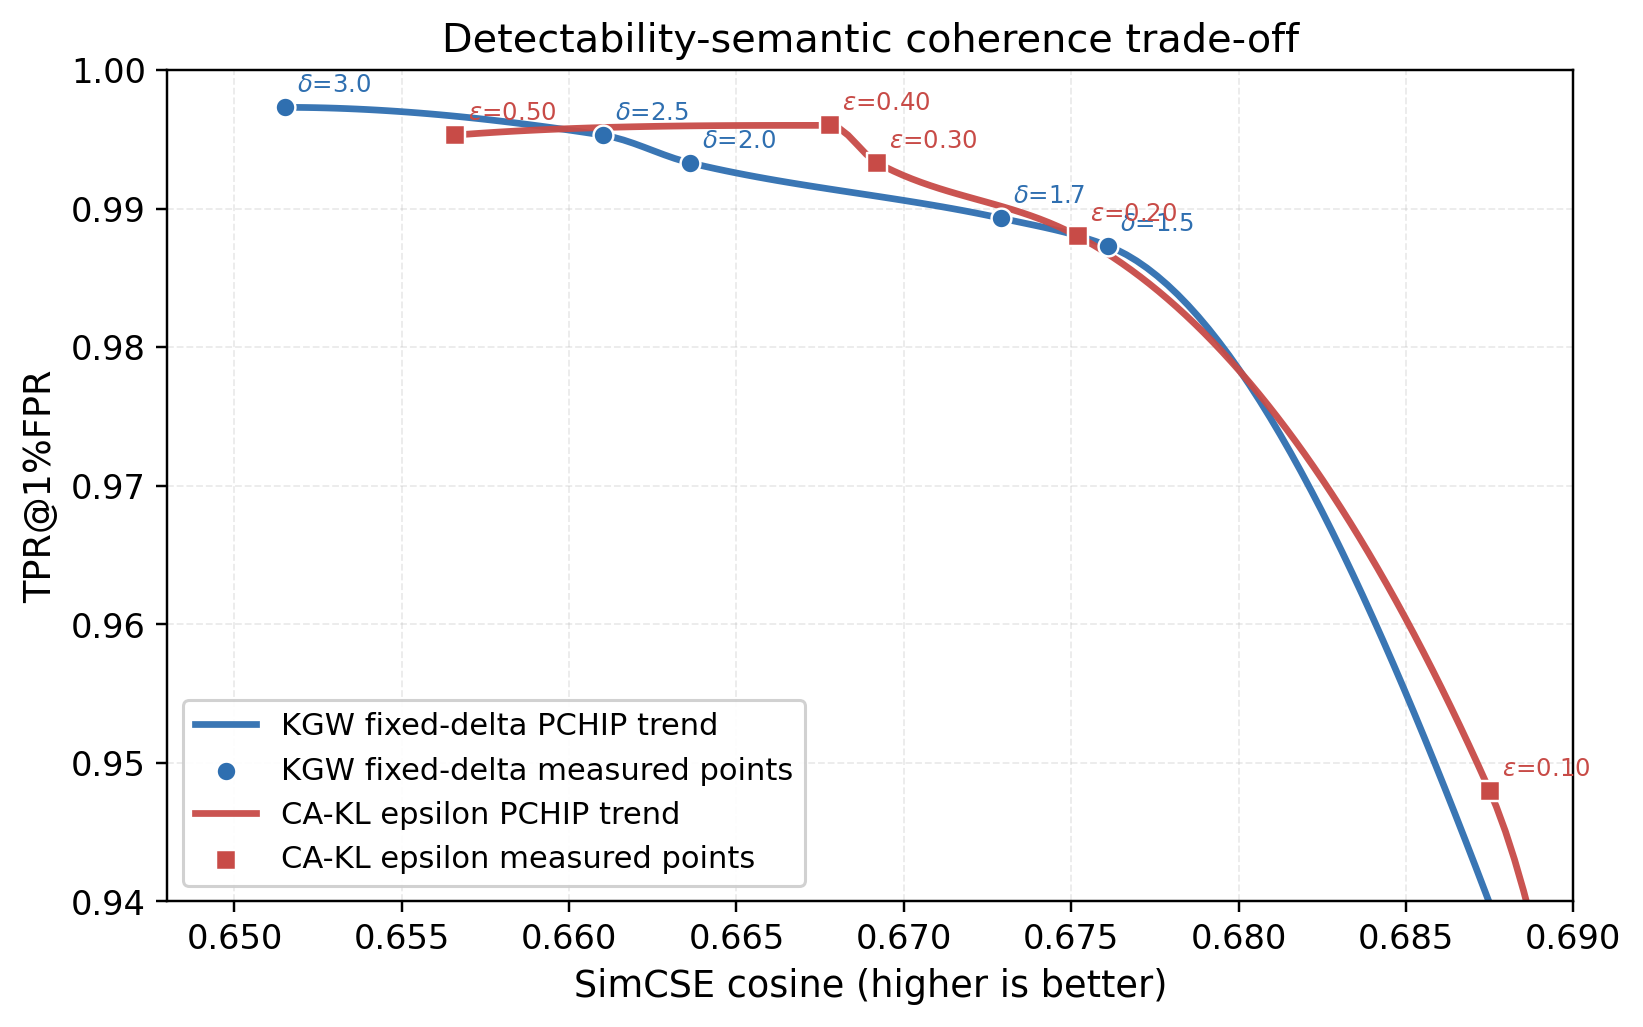
\includegraphics[width=0.93\textwidth]{simcse_vs_tpr_standard_kgw.png}
    \caption{Test-500 $\times$ 3 seeds 的 SimCSE--\tpr{} 高检测区。}
    \label{fig:sim-pareto}
\end{figure}

图~\ref{fig:ppl-pareto} 展示完整 corpus PPL--TPR 轨迹。PPL 越低越好，TPR 越高越好。随着 KGW $\delta$ 或 \cakl{} $\varepsilon$ 增大，两条曲线先快速提升检测率，随后在 99\% 附近饱和，而 PPL 仍继续增大。该图显示 \cakl{} 的 PPL 曲线并不严格优于 KGW：在 99.33\% TPR 处，\cakl{} $\varepsilon=0.30$ 的 corpus PPL 为 30.10，略高于 KGW $\delta=2.0$ 的 29.67；在更高检测区，\cakl{} $\varepsilon=0.50$ 与 KGW $\delta=2.5$ 的 TPR 均约为 99.5\%，corpus PPL 分别为 34.14 与 34.91，\cakl{} 略低。由此可见，\cakl{} 的主要收益不是无条件降低 PPL，而是在可解释 KL 预算下形成可控的检测--质量曲线，并在部分高检测工作点改善语义一致性指标。

\begin{figure}[H]
    \centering
    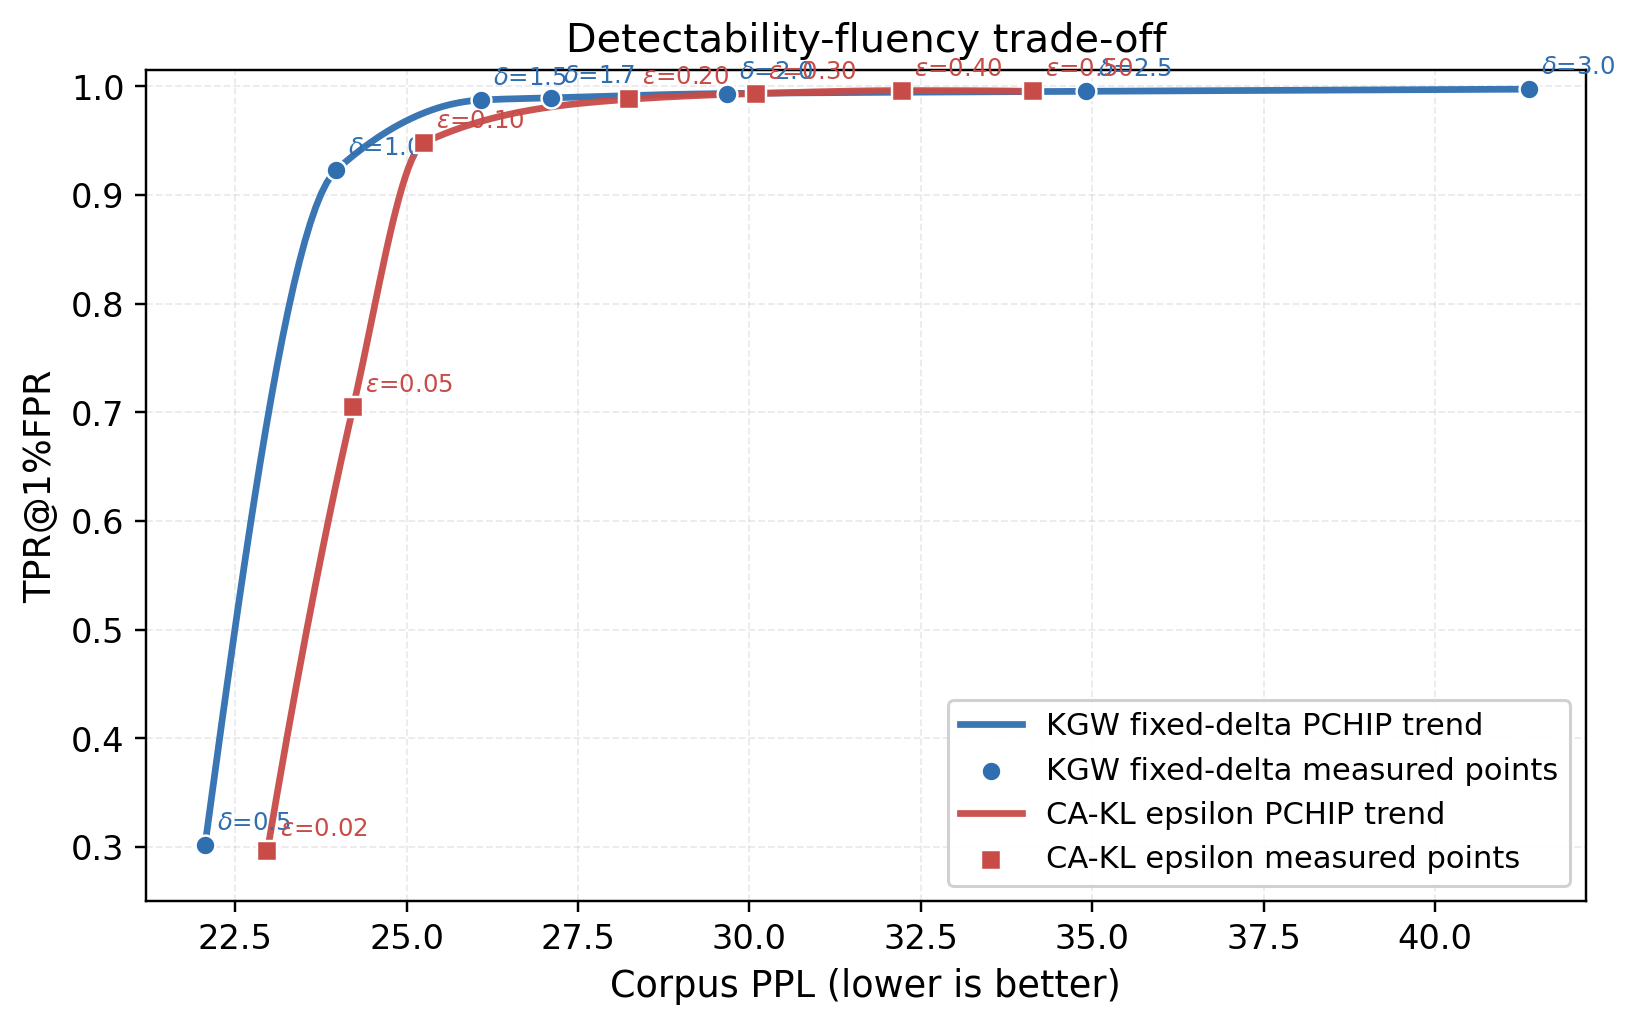
\includegraphics[width=0.93\textwidth]{ppl_vs_tpr_standard_kgw.png}
    \caption{Test-500 $\times$ 3 seeds 的 corpus PPL--\tpr{} 曲线。}
    \label{fig:ppl-pareto}
\end{figure}

综合 SimCSE 与 PPL，\cakl{} 在当前协议下相对 KGW 的改进可以概括为两点。第一，固定 $\delta$ 被逐 token KL 预算 $\varepsilon$ 取代，水印强度从经验偏置转化为可解释的分布约束，参数扫描形成更连续的折中曲线。第二，在部分高检测工作点，\cakl{} 可以在相同或接近的 TPR 下获得更高 SimCSE，例如 99.33\% TPR 处相对 KGW $\delta=2.0$ 的提升。与此同时，PPL 曲线与 KGW 仍有交错，bootstrap 区间也存在重叠，因此本文不宣称 \cakl{} 在 clean 条件下严格支配 KGW fixed-delta 包络，而将其定位为一种更可控的 token-specific 水印强度分配方法。

\subsection{完整方法与匹配检测}

根据 validation 结果，\caklcg{} 采用 $\varepsilon=0.10$、candidate top-p=0.95 和 90\% gate；其 test 实际 gate pass rate 为 88.94\%，平均 candidate size 为 298.2。matched fixed-delta control 使用 $\delta=1.5$ 和相同 candidate/gate，实际 gate pass rate 为 89.01\%。表~\ref{tab:matched} 展示 clean test 结果。

\begin{table}[H]
    \centering
    \caption{完整方法的 standard 与 matched detector 结果（目标 FPR 1\%，实际 human FPR 均为 0.6\%）}
    \label{tab:matched}
    \scriptsize
    \begin{tabularx}{\textwidth}{p{0.14\textwidth}p{0.20\textwidth}p{0.23\textwidth}p{0.15\textwidth}p{0.16\textwidth}}
        \toprule
        生成方法                & Detector                & TPR [95\% CI]                  & SimCSE & Corpus PPL \\
        \midrule
        \caklcg{}           & Standard KGW            & 86.40\% [84.40,88.47]          & 0.6897 & 21.27      \\
        \caklcg{}           & Matched weighted-global & \textbf{97.80\% [96.80,98.67]} & 0.6897 & 21.27      \\
        \caklcg{}           & Matched weighted-winmax & 89.33\% [87.67,91.00]          & 0.6897 & 21.27      \\
        \midrule
        KGW-CG $\delta=1.5$ & Standard KGW            & 97.73\% [96.67,98.67]          & 0.6820 & 20.66      \\
        KGW-CG $\delta=1.5$ & Matched weighted-global & \textbf{98.80\% [97.93,99.53]} & 0.6820 & 20.66      \\
        KGW-CG $\delta=1.5$ & Matched weighted-winmax & 98.60\% [97.60,99.40]          & 0.6820 & 20.66      \\
        \bottomrule
    \end{tabularx}
\end{table}

\caklcg{} 的 standard TPR 为 86.40\%，低于 \cakl{} base $\varepsilon=0.10$ 的 94.80\%。由于 standard detector 未重建 candidate 支持集与 gate，该差异反映的是生成--检测配置失配，而非水印证据的完全消失。matched weighted-global 达到 97.80\%，比 standard 高 11.40 个百分点，验证了检测配置匹配的必要性。Weighted-WinMax 在 clean 全文上的 TPR 低于 global；独立阈值校准控制了窗口搜索的多重比较效应，说明局部窗口聚合在全文水印场景中不必然提高检测功效。

与 matched KGW-CG 对照相比，\caklcg{} 的 SimCSE 高 0.0077，但 TPR 低 1.0 个百分点、corpus PPL 高 0.61，因此不存在单方面支配。该对照将完整系统的效应分解为动态 KL、candidate/gate 和 detector 三部分，避免将检测器增益直接归因于生成算法。

\section{总结}

本文从 KGW 复现出发，研究逐 token KL 约束水印及其 candidate/gate 扩展。实验采用结构化数据划分、全词表 greenlist、精确 continuation token 计分、检测器配置配对与 held-out 阈值校准；validation/test 各 500 条固定数据、三个 test seeds 和完整参数网格共同保证结果可比较。

test-500 $\times$ 3 seeds 表明，\cakl{} $\varepsilon=0.10$ 达到 94.80\% \tpr{}、0.6875 SimCSE 和 25.25 corpus PPL。该点与 KGW 包络接近，但不足以支持严格 Pareto 改进。完整方法 \caklcg{} 在 matched weighted-global detector 下达到 97.80\% TPR，明显高于其 standard 诊断值 86.40\%，证明匹配检测是 candidate/gate 系统不可缺少的组成部分。

因此，实验结果不支持 \cakl{} 在 clean 条件下全面优于 KGW，但支持以下方法贡献：逐 token KL 预算把水印强度转化为具有明确分布意义的约束；candidate/gate 与 matched detector 构成了清晰的联合生成--检测系统。上述结论由独立测试集上的检测率、SimCSE 与 corpus PPL 共同支持。

\section{实验分工}

\noindent\textbf{施煌：}负责 KGW 原论文阅读、官方仓库复现、C4 数据流程核对，以及报告中方法背景与复现部分的整理。

\noindent\textbf{祖裕柏：}负责本文改进水印生成端的主要实现与实验执行。具体包括在 KGW logits processor 基础上实现 \cakl{} 逐位置 KL 预算求解，将固定 $\delta$ 改为按当前位置分布自适应选择的 $\delta_t$；设计并实现 candidate-aware greenlist，使水印划分限制在当前 top-p 候选集合内；实现基于 entropy/top-1 条件的 confidence gate，控制哪些生成位置参与嵌入；编写批量生成脚本，完成 KGW fixed-delta、\cakl{} epsilon 网格、candidate-only、gate-only 与 candidate+gate 等方法的 validation 参数扫描和 test 集独立生成，并整理生成结果、运行日志与实验配置。

\noindent\textbf{黄镇邦：}负责检测端、离线评测与结果分析的主要工作。具体包括实现 standard KGW detector 以及与 candidate/gate 配置一致的 matched weighted-global、matched weighted-winmax detector；设计 validation human completions 上的低 FPR 阈值校准流程，并在 test human completions 上核对实际误报率；完成 continuation-only corpus PPL 与 prompt/seed 配对 SimCSE 评测，保证质量指标只作用于生成 continuation；编写 prompt-cluster bootstrap 统计脚本，估计 TPR、SimCSE 与 PPL 的 95\% 置信区间；绘制检测率--语义一致性、检测率--PPL 折中曲线和完整方法对比表，并负责报告中实验结果、统计解释和结论边界的撰写。

\clearpage
\bibliographystyle{ieeetr}
\bibliography{reference}

\end{document}
